\section{Folgen und Reihen}

\begin{center}
    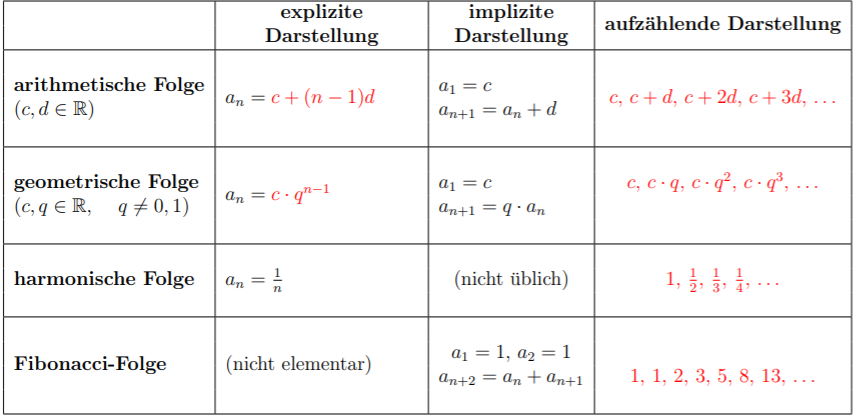
\includegraphics[width=1\linewidth]{images/folgenreihen.png}
\end{center}

\subsection{Grenzwerte von Folgen}
\subsubsection{Beschränkte Folge}
Eine Folge $(a_n)$ heisst beschränkt, falls es eine positive reele Zahl $M$ gibt, so dass gilt: $|a_n| \leq M$ für alle $n \in \mathbb{N}$. Falls dies nicht der Fall ist, heisst die Folge unbeschränkt. \\
Eine Folge $(a_n)$ heisst nach unten bzw. nach oben beschränkt, falls es eine reele Zahl $m$ bzw. $M$ gibt mit $m \leq a_n$ bzw. $a_n \leq M$ für alle $n \in \mathbb{N}$.

\subsubsection{Grenzwert, formale Definition}
Eine reelle Zahl $g$ heisst Grenzwert oder Limes der Folge $(a_n)$, wenn es zu jedem $\epsilon > 0$ eine natürliche Zahl $n_0$ gibt, so dass für alle $n\geq n_0$ stets $|a_n - g| < \epsilon$ gilt. \\
Eine Folge heisst konvergent, wenn sie einen Grenzwert $g$ hat.

\subsection{Rechnen mit Grenzwerten}
\begin{align}
    &\lim_{n \rightarrow \infty}(c \cdot a) = c \cdot \lim_{n \rightarrow \infty} a_n
\end{align}
\begin{align}
    &\lim_{n \to \infty} (a_n \cdot b_n) = \lim_{n \to \infty} (a_n) + \lim_{n \to \infty} (b_n)
\end{align}
\begin{align}
    &\lim_{n \to \infty} (a_n \cdot b_n) = \lim_{n \to \infty} (a_n) \cdot \lim_{n \to \infty} (b_n)
\end{align}
\begin{align}
    &\lim_{n \to \infty} (\frac{a_n}{b_n}) = \frac{\lim_{n \to \infty} (a_n)}{\lim_{n \to \infty} (b_n)}, \lim_{n \to \infty}(b_n) \neq 0, b \neq 0
\end{align}

\vfill

\subsubsection{Rationale Funktion - Grenzwert bestimmen}
\begin{enumerate}
    \item Bruch mit der höchsten Potenz von $n$, die vorkommt kürzen
    \item Das Verhalten der einzelnen Summanden für $n \to \infty$ untersuchen.
    \item Grenzwert bestimmen
\end{enumerate}

\textbf{Fall 1 } Zählergrad < Nennergrad: \[\lim_{n \to \infty} \frac{g(n)}{h(n)} = 0\] \\
\textbf{Fall 2 } Zählergrad > Nennergrad: \[\frac{g(n)}{h(n)} \to \infty \] \\
\textbf{Fall 1 } Zählergrad = Nennergrad: \[\lim_{n \to \infty} \frac{g(n)}{h(n)} = \frac{\text{führender Term von }g}{\text{führender Term von } h}\] \\

\textbf{Eine spezielle Folge: } $(1+\frac{1}{n})^n$ strebt gegen $e$.

\subsubsection{Summenfolge}
Die Summenfolge oder Reihe $s$ der reellen Folge $a$ ist definiert durch:
\begin{align*}
    &s_1 = a_1 \\
    &s_2 = a_1 + a_2\\
    &s_2 = a_1 + a_2 + a_3\\
    &s_2 = a_1 + a_2 + a_3 + a_4\\
    &\vdots \\
    &s_n = a_1 + a_2 + \dots + a_n = \sum_{k=1}^{n}a_k
\end{align*}

\subsubsection{Arithmetische Reihe}
Bei einer arithmetischen Folge ist die Differenz zweier aufeinanderfolgender Flieder konstant. \\
Die Summe der ersten $n$ Elemente einer arithmetischen Folge ist:
\[
    s_n = n \cdot a_1 + \frac{n(n-1)}{2} \cdot 3
\]

\subsubsection{Geometrische Reihe}
Bei einer geometrischen Folge ist der Quotient zweier aufeinanderfolgenden Glieder Konstant. \\
Die Summe der ersten $n$ Elemente einer geometrischen Folge ist:
\[
    s_n = \frac{a_1(q^n-1)}{q-1} = \frac{a_1(1-q^n)}{1-q}
\]

\subsection{Grenzwerte von Reihen}
Für den Grenzwert der Reihe $s$ einer reellen Folge $a$ schreiben wir:
\[
    g=\lim_{n \to \infty} s_n = \sum_{l=1}^{\infty}a_k
\]

\subsubsection{Grenzwert einer arithmetischen Reihe}
\textbf{Jede arithmetische Reihe divergiert.}

\subsubsection{Grenzwert einer geometrischen Reihe}
Wie verhält sich $s_n = a_1 \cdot \frac{1-q^n}{1-q}$, wenn $n \to \infty$ \\
\textbf{Fall 1 } $q>1$ \hspace{5em} Die Reihe strebt gegen $\infty$ oder $-\infty$ hat aber keinen Grenzwert. \\
\textbf{Fall 2 } $q\leq -1$ \hspace{5em} Die Reihe strebt zwischen positiven und negativen Werten hin und her und hat keinen Grenzwert \\
\textbf{Fall 3 } $|q|<1$ \hspace{5em} Die Reihe strebt gegen den Grenzwert $\frac{a_1}{1-q}$. Sie konvergiert also.

\section{Grenzwert und Stetigkeit einer Funktion}
\subsection{Grenzwert einer Funktion im Endlichen}
\subsubsection{Rechenregeln}
\begin{align*}
    &\lim_{x \to x_0} (c \cdot f(x)) = c \cdot (\lim_{x \to x_0} f(x)) \\
    &\lim_{x \to x_0}(f(x)+g(x)) = \lim_{x \to x_0}f(x) + \lim_{x \to x_0} g(x) \\
    &\lim_{x \to x_0} (f(x)-g(x)) = \lim_{x \to x_0} f(x) + \lim_{x \to x_0} g(x) \\
    &\lim_{x \to x_0} (f(x) \cdot g(x)) = (\lim_{x \to x_0} f(x)) \cdot (\lim_{x \to x_0} g(x)) \\
    &\lim_{x \to x_0} \frac{f(x)}{g(x)} = \frac{\lim_{x \to x_0} f(x)}{\lim_{x \to x_0} g(x)}
\end{align*}

\subsubsection{Stetigkeit von Funktionen}
Eine Funktion $f(x)$ heisst stetig an der Stelle $x_0$, wenn der Grenzwert $\lim_{x \to x_0} f(x)$ existiert und $= f(x_0)$ ist. \\
Eine Funktion heisst stetig, wenn sie an jeder Stelle ihres Definitionsbereiches stetig ist. \\
Die Summe, die Differenz, das Produkt, die Komposition von stetigen Funktionen sind stetig.
\\
Falls eine Funktion $f(x)$ auf einem Intervall $[a,b]$ stetig ist, und $f(a)$ und $f(b)$ verschiedene Vorzeichen haben, dann hat $f$ in $[a,b]$ mindestens eine Nullstelle.
\subsubsection{Grenzwerte von gebrochenrationalen Funktionen}
\begin{center}
    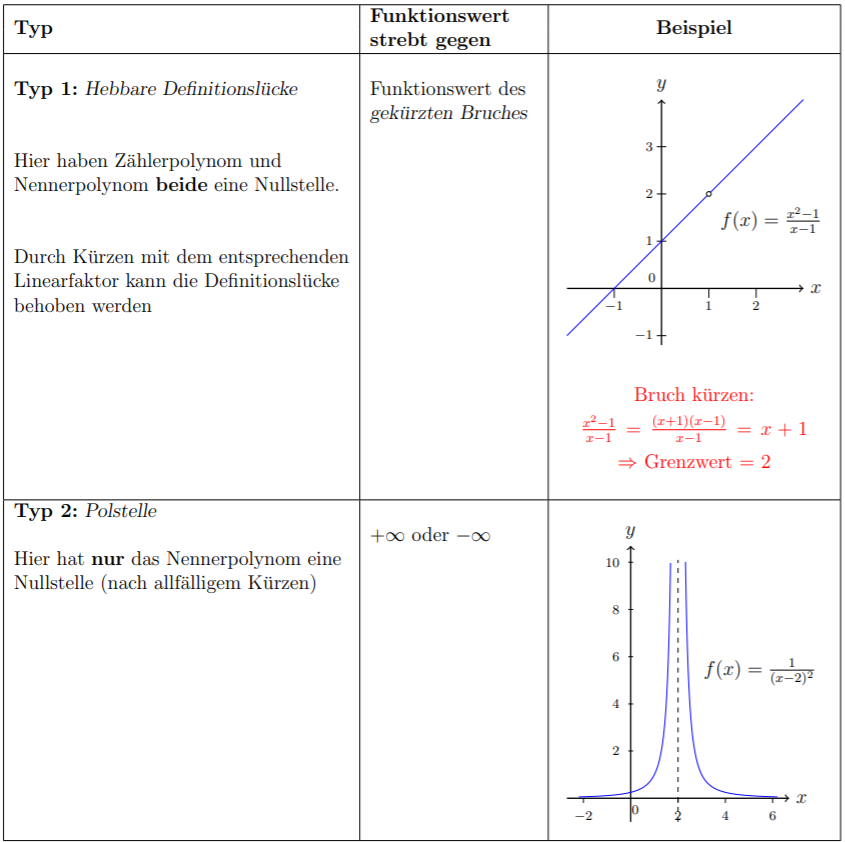
\includegraphics[width=1\linewidth]{images/grenzrational.png}
\end{center}